\section{Metodología}
\label{sec:metodologia} 

Para alcanzar el objetivo general y los objetivos específicos planteados en la Sección \ref{sec:objetivos}, se adopta una metodología de \textbf{Prototipado Evolutivo}. Este enfoque es adecuado para proyectos de ingeniería que involucran hardware y software, ya que permite el desarrollo, prueba y refinamiento de un sistema funcional de manera incremental y controlada.

La metodología se estructura en cinco fases principales, las cuales se describen a continuación y se ilustran conceptualmente en la Figura \ref{fig:fases_metodologia}.

\begin{figure}[H]
    \centering
    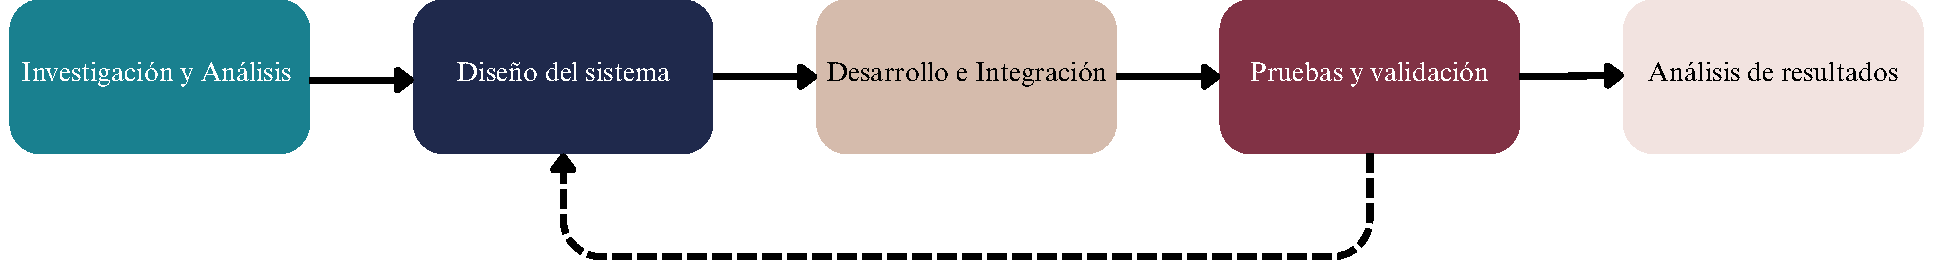
\includegraphics[width=0.9\linewidth]{Documento/Imagenes/Metodologia/fases_proyecto.pdf}
    \caption{Fases de la metodología de prototipado evolutivo adoptada, mostrando el ciclo de refinamiento.}
    \label{fig:fases_metodologia}
\end{figure}

\subsection{Fase 1: Investigación y Análisis de Requerimientos} 
\label{subsec:met_fase1} 
Esta fase inicial establece las bases conceptuales y técnicas del proyecto. Comprende:
\begin{itemize}
    \item \textbf{Revisión del Estado del Arte:} Investigación de trabajos previos y soluciones existentes para identificar el contexto tecnológico y las oportunidades de innovación.
    \item \textbf{Establecimiento del Marco Teórico:} Fundamentación de los conceptos clave en áreas como redes de sensores, comunicaciones inalámbricas, visión artificial y gestión de datos.
    \item \textbf{Definición de Requerimientos:} Traducción de las necesidades del problema en un conjunto formal de Requerimientos Funcionales y No Funcionales, que guiarán el diseño y la validación.
\end{itemize}

\subsection{Fase 2: Diseño de la Arquitectura y Selección de Tecnologías} 
\label{subsec:met_fase2} 
Basándose en los requerimientos definidos, esta fase consiste en el análisis de ingeniería para tomar las decisiones de diseño del prototipo.
Las actividades incluyen:
\begin{itemize}
    \item Diseño de la arquitectura general del sistema.
    \item Análisis comparativo y selección de los componentes de hardware.
    \item Análisis comparativo y selección de las tecnologías de comunicación y la topología de red.
    \item Diseño de la arquitectura de software en el servidor y selección de la plataforma.
    \item Selección y justificación del modelo y la arquitectura específica para la visión artificial.
\end{itemize}
El resultado de esta fase es la especificación técnica detallada del prototipo.

\subsection{Fase 3: Desarrollo e Integración del Prototipo} 
\label{subsec:met_fase3} 
Fase de implementación donde las especificaciones de diseño se materializan en un sistema funcional. Incluye:
\begin{itemize}
    \item Desarrollo de Hardware (ensamblaje, encapsulado).
    \item Desarrollo de Firmware (programación de MCUs).
    \item Desarrollo de Backend (configuración servidor, BD, API).
    \item Entrenamiento/Afinamiento del Modelo de IA.
    \item Desarrollo de Frontend (aplicación web).
\end{itemize}

\subsection{Fase 4: Pruebas y Validación} 
\label{subsec:met_fase4} 
El objetivo es verificar que el prototipo cumple con los requerimientos. Se aplicarán pruebas en distintos niveles:
\begin{itemize}
    \item Pruebas Unitarias.
    \item Pruebas de Integración.
    \item Pruebas del Sistema (Alfa) en entorno controlado.
    \item Pruebas de Campo (Piloto) en entorno real, con posible retroalimentación al diseño.
\end{itemize}

\subsection{Fase 5: Análisis de Resultados y Documentación}
\label{subsec:met_fase5} 
La fase final del proyecto se centra en:
\begin{itemize}
    \item Recolección y análisis de los datos de las pruebas.
    \item Evaluación objetiva del rendimiento del prototipo (presentado en el capítulo de Resultados).
    \item Discusión de limitaciones y trabajo futuro.
    \item Elaboración de conclusiones.
    \item Consolidación de todo el proceso en el presente documento de tesis.
\end{itemize}
